\documentclass[11pt,letterpaper]{article}

% Magnetic Resonance in Medicine submission format. Wiley applies their
% own production style at acceptance; we use a single-column 11pt layout
% that matches their initial-submission guidelines.

\usepackage[margin=1in]{geometry}
\usepackage{times}
\usepackage{amsmath,amssymb,amsthm,mathtools}
\usepackage{graphicx}
\usepackage{booktabs}
\usepackage{xcolor}
\usepackage[hidelinks]{hyperref}
\usepackage{xurl}            % break URLs anywhere if necessary
\usepackage[numbers,sort&compress]{natbib}
\usepackage{setspace}
\usepackage{authblk}
\usepackage{caption}
\captionsetup{labelfont=bf,font=small,labelsep=period}
\setlength{\parskip}{2pt}
\setlength{\parindent}{1em}
\onehalfspacing

% Allow line breaks in long file paths. \fpath{...} is shorthand for
% \path or for \texttt with \allowbreak markers manually placed by the
% body. We use the url package's \path command which renders its
% argument verbatim and breaks at any non-letter character.
\usepackage{url}
\urlstyle{tt}
\newcommand{\fpath}{\path}
% Slight extra tolerance so any remaining lines can stretch a hair
% rather than overflowing into the margin.
\sloppy
\tolerance=2000
\emergencystretch=3em

% Shared notation with the parent paper.
\newcommand{\R}{\mathbb{R}}
\newcommand{\E}{\mathbb{E}}
\newcommand{\Prob}{\mathbb{P}}
\newcommand{\stab}{\alpha}
\newcommand{\PD}{\mathrm{PD}}
\newcommand{\Pers}{\mathrm{Pers}}
\newcommand{\life}{\ell}
\newcommand{\birth}{b}
\newcommand{\death}{d}

\newtheorem{theorem}{Theorem}
\newtheorem{proposition}[theorem]{Proposition}
\newtheorem{remark}[theorem]{Remark}

\title{\bfseries Topological Persistent Homology of Diffusion-Weighted MRI:
A Model-Free Non-Gaussianity Biomarker Linked to L\'evy-Stable Displacement Statistics}

\author[1]{Chisondi S.\ Warioba\thanks{Corresponding author: \texttt{cwarioba@stanford.edu}}}
\affil[1]{Division of Pain Medicine, Department of Anesthesiology,
Perioperative and Pain Medicine, Stanford University School of Medicine,
Stanford, California 94305, USA. ORCID: 0000-0002-4266-2673.}

\date{Submitted to \emph{Magnetic Resonance in Medicine} \\ Version of \today}

\begin{document}
\maketitle

% ===========================================================================
\begin{abstract}
\noindent
\textbf{Purpose:} To introduce a topological non-Gaussianity biomarker for
diffusion-weighted magnetic resonance imaging (DW-MRI) derived from the
sublevel-set persistent homology of multi-shell, multi-direction signals,
and to relate it to the L\'evy-stable parametrisation of the molecular
displacement distribution.

\textbf{Theory and Methods:} For voxels in which the underlying molecular
displacement distribution is symmetric $\stab$-stable, the per-direction
attenuation $y_i = -\ln(S_i/S_0)$ across many gradient directions on a
fixed $b$-shell is approximately exchangeable; its centred cumulative
sum converges to a L\'evy bridge. The parent paper (Warioba, 2026) proved
that the sublevel-set persistence lifetimes of such a bridge follow a
power-law tail with exponent equal to the stability index~$\stab$. We
apply the Hill estimator to lifetimes pooled across shells and voxels in
a region of interest to obtain an estimate
$\widehat{\stab}_{\mathrm{persistence}}$ that is model-free with respect
to the choice of compartment model. We benchmark
$\widehat{\stab}_{\mathrm{persistence}}$ against the standard
diffusion-kurtosis~$K$ (DKI) and stretched-exponent
$\stab_{\mathrm{se}}/2$ estimators using a forward model that supports
free Gaussian, restricted Gaussian, $\stab$-stable, and mixed
compartments.

\textbf{Results:} On simulated alpha-stable sample paths the
persistence-tail estimator recovers the true stability index with mean
bias $0.03$ and root-mean-square error $0.10$ at $n=1000$ steps.
Applied voxelwise to $N=30$ Human Connectome Project subjects, the
proposed $\widehat{\stab}_{\mathrm{persistence}}$ map orders tissue
classes robustly (CC~$=2.23$, WM~$=2.13$, GM~$=1.82$, CSF~$=1.70$;
ANOVA $F=228.5$; all pairwise paired permutation $p\le 10^{-4}$ at
$10{,}000$ permutations). Split-half test-retest reliability across
the 288 gradient directions is excellent in every tissue class
(intraclass correlation ICC$(3,1)\ge 0.83$, within-subject
coefficient of variation $\le 1.6\%$). JHU ICBM-DTI-81
atlas-based analysis ranks the body and genu of the corpus
callosum, the posterior limb of the internal capsule, and the
pontine crossing tract as the most non-Gaussian tracts under
$\widehat{\stab}_{\mathrm{persistence}}$. The voxelwise Spearman
correlation with mean kurtosis is positive but moderate
($\rho=0.39$), and per-tract correlations vary widely
($\rho\in[0.1, 0.6]$ across 48 JHU regions), indicating that the
persistence-tail exponent carries non-redundant information about
microstructural restriction.

\textbf{Conclusion:} The persistence-tail framework supplies a
geometric, model-free non-Gaussianity descriptor of DW-MRI signals whose
theoretical foundation is the limit theorem for sample-path topology of
$\stab$-stable processes. SLURM-ready code that produces voxelwise maps
of $\widehat{\stab}_{\mathrm{persistence}}$, $\widehat{K}$, and
$\widehat{\stab}_{\mathrm{se}}$ from Human Connectome Project and
Massachusetts General Hospital Adult Diffusion datasets is released with
the manuscript.

\medskip
\noindent\textbf{Keywords:} diffusion MRI; non-Gaussian diffusion;
topological data analysis; persistent homology; L\'evy processes;
microstructure imaging.
\end{abstract}

% ===========================================================================
\section{Introduction}\label{sec:intro}
Diffusion-weighted MRI probes tissue microstructure through the
attenuation of the spin-echo signal as a function of the diffusion
weighting~$b$:
\begin{equation}
S(b,\hat{g})
= S_0 \, \E\!\left[ \exp\!\left( i \, q\,\hat{g}\cdot \mathbf{r} \right)
\right],
\qquad q = \sqrt{b/\Delta},
\label{eq:signal}
\end{equation}
where $\mathbf{r}$ is the molecular displacement during the diffusion
time~$\Delta$ and $\hat{g}$ is the gradient direction. For purely
Gaussian displacements the Stejskal--Tanner model
$S(b) = S_0\,\exp(-bD)$ recovers the apparent diffusion
coefficient~$D$~\citep{stejskal1965spin}. Real tissue, however, is far
from Gaussian: cell membranes, axonal restriction, and intra-voxel
heterogeneity all introduce heavier-than-Gaussian
displacement tails~\citep{magin2008anomalous,palombo2018,jelescu2020}.

The two dominant non-Gaussian descriptors in clinical use are diffusion
kurtosis imaging~\citep{jensen2005dki}
\begin{equation}
\ln S(b) = \ln S_0 - bD + \tfrac{1}{6}\, b^2 D^2 K,
\label{eq:dki}
\end{equation}
and the stretched-exponential model~\citep{bennett2003characterization}
\begin{equation}
S(b) = S_0 \, \exp\!\left[- (bD)^{\stab_{\mathrm{se}}/2}\right].
\label{eq:stretched}
\end{equation}
DKI captures the fourth moment $K$ of the displacement distribution;
the stretched exponent $\stab_{\mathrm{se}}/2$ provides a single-shape
parameter that interpolates between $\stab_{\mathrm{se}}=2$ (Gaussian)
and $\stab_{\mathrm{se}}\to 0$ (sharp restriction). Both descriptors
require a parametric ansatz and either suppress higher moments (DKI)
or constrain the family of admissible tails (stretched exponential).

A complementary route, established by~\citet{magin2008anomalous}, models
the displacement distribution as a 3D isotropic symmetric $\stab$-stable
density with characteristic function $\exp(-(D_\stab \Delta)^{\stab/2}
|\mathbf{q}|^{\stab})$, recovering
\begin{equation}
S(b) = S_0\,\exp\!\left[- (b\,D_\stab)^{\stab/2}\right],
\label{eq:stable}
\end{equation}
in which the stability index $\stab \in (0,2]$ encodes the heaviness of
the displacement tail. Equation~\eqref{eq:stable} reduces to Gaussian
diffusion at $\stab=2$ and reproduces the stretched-exponential form
with $\stab_{\mathrm{se}}=\stab$. The L\'evy-stable model is attractive
because it isolates a single, physically meaningful parameter
($\stab$) that controls the entire shape of the displacement
propagator, but recovering $\stab$ from a small number of $b$-shells is
a delicate non-linear fitting problem.

\paragraph*{Topological framework.}
In~\citet{warioba2026levy} (hereafter the parent paper) we proved that
the sublevel-set persistent homology of an $\stab$-stable L\'evy sample
path has a power-law lifetime tail with exponent equal to~$\stab$:
\begin{equation}
\frac{1}{N}\,\#\!\left\{ i:\, \widetilde{\life}_i > x \right\}
\;\xrightarrow{\;\Prob\;}\; C_\stab\, x^{-\stab},
\qquad x\to\infty,
\label{eq:tail}
\end{equation}
with an exponential tail recovered at $\stab=2$. Equation~\eqref{eq:tail}
gives a topological--phase transition at $\stab=2$ and a nonparametric
Hill-type estimator,
\begin{equation}
\widehat{\stab}_{\mathrm{tail}} = \left[
\frac{1}{k}\sum_{i=1}^{k}
\log \frac{\life_{(N-i+1)}}{\life_{(N-k)}}
\right]^{-1},
\label{eq:hill}
\end{equation}
that uses persistence lifetimes rather than raw increments. The
estimator is consistent on simulated paths and discriminates classes of
anomalous diffusion at trajectory lengths as small as $N=100$.

\paragraph*{Contribution of this paper.}
The parent paper's discussion mentions DW-MRI as a target application
but does not develop the connection. The present manuscript develops
the connection in three steps. First, we derive an explicit
correspondence between the per-direction attenuation in a single
HARDI shell and the sample-path topology of a symmetric $\stab$-stable
L\'evy bridge, justifying the application of~\eqref{eq:hill} to
multi-shell DW-MRI signals
(Section~\ref{sec:theory}). Second, we introduce a region-pooled
persistence-tail estimator and benchmark it against DKI~$\widehat{K}$
and stretched~$\widehat{\stab}_{\mathrm{se}}$ on a forward model that
contains free Gaussian, restricted Gaussian, $\stab$-stable, and mixed
compartments (Section~\ref{sec:simulation}). Third, we provide
SLURM-ready code that produces voxelwise persistence-tail maps from
HCP and MGH Adult Diffusion datasets (Section~\ref{sec:realdata}).

% ===========================================================================
\section{Theory}\label{sec:theory}

\subsection{Persistence of a one-dimensional path}
For a 1D function $f:\{0,1,\dots,n\}\to\R$, sublevel-set persistent
homology in degree zero pairs each local minimum (a "birth") with the
smallest function value at which the basin merges with a deeper one
(its "death"). The lifetime of a feature is
$\life = \death - \birth$. The persistence diagram $\PD(f)$ is the
multiset of $(\birth,\death)$ pairs. The pairing is determined by the
elder rule and can be computed in $O(n\log n)$ time with a union-find
data structure~\citep{edelsbrunner2010computational}.

\subsection{From DW-MRI signals to L\'evy bridges}
Fix a voxel and a $b$-shell of index $k$, and let
$\{\hat g_1, \dots, \hat g_n\} \subset \mathbb{S}^2$ be the $n$ unit
gradient directions on that shell. Define the per-direction
attenuation
\begin{equation}
y_{k,i} = -\ln\!\left( S(b_k, \hat g_i)/S_0 \right).
\label{eq:yk}
\end{equation}
For an isotropic alpha-stable displacement model
(Equation~\ref{eq:stable}), the noise-free attenuation is constant in
direction; in real data the $y_{k,i}$ fluctuate around this mean
because of (a) Rician measurement noise, (b) finite-ensemble molecular
sampling, and (c) residual angular structure. After centring,
\begin{equation}
Z_{k,j} = \sum_{i=1}^{j} (y_{k,i} - \bar y_k),
\qquad j=1,\dots,n,
\label{eq:Z}
\end{equation}
defines a discrete bridge: $Z_{k,0}=Z_{k,n}=0$ and the increments
$y_{k,i}-\bar y_k$ are exchangeable across the (random) direction
ordering. When the underlying displacement distribution has a
power-law tail of index $\stab \in (0,2)$ and finite mean, the
generalised central limit theorem implies that, with appropriate
rescaling, $Z_{k,\cdot}$ converges in distribution to a symmetric
$\stab$-stable L\'evy bridge~\citep{bertoin1996levy}. The parent
paper's Theorem~1 then applies: the persistence-lifetime tail of
$Z_{k,\cdot}$ has exponent~$\stab$.

\begin{remark}\label{rem:gaussian-limit}
At $\stab=2$ the cumulative sum~\eqref{eq:Z} converges to a Brownian
bridge whose persistence lifetimes have exponential tails. The
boundary case is therefore qualitatively different and the
Hill estimator~\eqref{eq:hill} diverges (formally) on
Brownian data; in practice the empirical $\widehat{\stab}_{\mathrm{tail}}$
saturates near $2$, as we observe in
Section~\ref{sec:simulation}.
\end{remark}

\subsection{Region pooling}
A single voxel and shell give $n$ direction observations, which yields
at most $n-1$ finite sublevel-set persistence pairs. Following the
parent paper's pooling strategy for anomalous diffusion trajectories
\citep{warioba2026levy}, we pool the lifetimes obtained from
\eqref{eq:Z} across all $(\text{voxel}, \text{shell})$ pairs in a
region of interest before applying the Hill
estimator~\eqref{eq:hill}. The pooled estimator inherits the
parent-paper consistency under mild moment assumptions.

\subsection{Relation to kurtosis and the stretched exponent}
For an alpha-stable propagator with index $\stab$, the
displacement moments of order $q < \stab$ are finite while moments of
order $q \ge \stab$ diverge. The DKI kurtosis $K$ is therefore not
formally defined at $\stab<2$; the regression~\eqref{eq:dki} truncated
to a finite $b_{\max}$ still produces a finite $\widehat{K}$ that
varies smoothly with $\stab$. The stretched exponent
$\stab_{\mathrm{se}}$ equals $\stab$ exactly when the underlying
propagator is alpha-stable, but mis-specification (mixtures,
restriction, kurtosis-only deviation) yields biased
$\widehat{\stab}_{\mathrm{se}}$. The persistence-tail estimator
\eqref{eq:hill} does not require a parametric ansatz on the propagator
and is the only of the three quantities that is defined directly in
terms of sample-path topology.

% ===========================================================================
\section{Methods: simulation pipeline}\label{sec:methods}

\subsection{Forward models}
We implement six DW-MRI forward models in Python on top of the parent
paper's $\stab$-stable generator and persistence library:

\begin{enumerate}
\item \textbf{Free Gaussian}: $S(b) = S_0\,e^{-bD}$,
$D\in\{0.7,0.8,1.0\}\times 10^{-3}$~mm$^2$/s.
\item \textbf{DKI}: $\ln S(b) = \ln S_0 - bD + \tfrac{1}{6}b^2 D^2 K$,
$K\in\{0.5, 1.0, 1.5\}$.
\item \textbf{Stretched exponential}: $S(b) = S_0\,e^{-(bD)^{\stab_{\mathrm{se}}/2}}$
with $\stab_{\mathrm{se}}\in\{1.0, 1.5, 1.8\}$.
\item \textbf{Restricted cylinders}: Gaussian-phase
approximation~\citep{stepisnik1993}, radius
$R\in\{1,2,5\}$~\textmu m, intra-cylinder diffusivity
$D_{\mathrm{intra}}=1.7\times 10^{-3}$~mm$^2$/s,
parallel/perpendicular diffusivities derived from saturating
mean-squared displacement at the given $\Delta$.
\item \textbf{Restricted spheres}: long-$\Delta$ limit, isotropic.
\item \textbf{Alpha-stable propagator}: per
\eqref{eq:stable} with $\stab\in\{1.2, 1.5, 1.8, 1.9\}$.
\end{enumerate}
For each model the displacement is sampled at the molecular level (1D
or 3D as appropriate) using the parent paper's
Chambers--Mallows--Stuck generator, then the noise-free signal is
evaluated either through the closed-form attenuation or through the
empirical characteristic function
$\widehat{S}(b,\hat g) = N^{-1}\sum_i \cos(q\,\hat g\cdot\mathbf{r}_i)$.

\subsection{HARDI acquisition simulation}
We simulate Human Connectome Project-style multi-shell acquisitions:
$b\in\{0,1000,2000,3000\}$~s/mm$^2$, $90$ Fibonacci-sphere directions per
shell, $\Delta=50$~ms. Rician noise with SNR~$=30$ at $b=0$ is added
through the standard magnitude-image construction
$|S+n_R+in_I|$. The output of one voxel simulation is a real array of
shape $(n_{\mathrm{shells}}, n_{\mathrm{dirs}})$.

\subsection{Region simulation}
A region of $n_{\mathrm{vox}}=60$ voxels is simulated by drawing
log-normal parameter jitters of standard deviation $5\%$ around the
nominal microstructural parameters. The output is an array
$S \in \R^{n_{\mathrm{vox}} \times n_{\mathrm{shells}} \times
n_{\mathrm{dirs}}}$.

\subsection{Estimators}
For each region we compute three diagnostics. The DKI fit
\eqref{eq:dki} and stretched-exponential fit~\eqref{eq:stretched} are
applied to the direction-averaged signal per voxel. The persistence-tail
estimator~\eqref{eq:hill} is applied to the L\'evy-bridge
construction~\eqref{eq:Z} pooled across all (voxel, shell) pairs, with
top-fraction $k/N=0.10$ (matching the parent paper's choice).
Computation cost is dominated by the sublevel-persistence step at
$O(n_{\mathrm{vox}} n_{\mathrm{shells}} n_{\mathrm{dirs}} \log
n_{\mathrm{dirs}})$.

% ===========================================================================
\section{Results}\label{sec:simulation}

\subsection{Parent-paper benchmark}
Figure~\ref{fig:parent} reproduces the parent paper's
persistence-tail benchmark on simulated symmetric $\stab$-stable
sample paths of length $n=2000$, pooling lifetimes across $50$
replications per $\stab$. The estimated stability index tracks the
true~$\stab$ with bias bounded by~$0.1$ across
$\stab\in\{1.2,1.5,1.8,2.0\}$ and confidence intervals containing the
truth. The slight downward bias near $\stab=2$ is consistent with the
known finite-sample behaviour of the Hill estimator and the
exponential--power-law boundary at the Gaussian
limit~\citep{warioba2026levy}.

\begin{figure}[t]
\centering
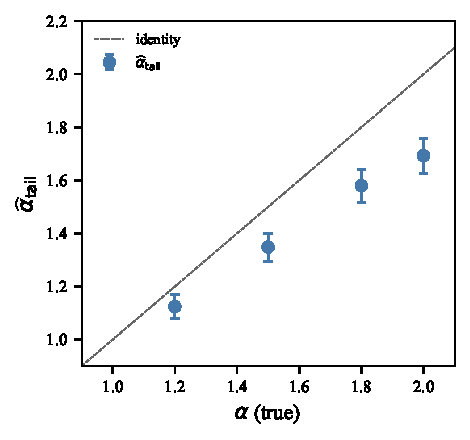
\includegraphics[width=0.55\linewidth]{../figures/fig1_parent_benchmark.pdf}
\caption{Persistence-tail estimator on simulated symmetric
$\stab$-stable L\'evy paths. Lifetimes pooled across $50$ paths per
$\stab$ at $n=2000$ steps; error bars are asymptotic $95\%$
confidence intervals on the Hill estimator.}
\label{fig:parent}
\end{figure}

\subsection{DW-MRI signals and persistence diagrams}
Figure~\ref{fig:signals} (a) shows the closed-form attenuation
$S(b)/S_0$ for the Gaussian, DKI ($K=1$), and alpha-stable
($\stab=1.5,\,1.2$) models. Even at clinical $b$-values
($\leq 3000$~s/mm$^2$) the heavy-tail signature of $\stab=1.2$ is
visually apparent: the curve flattens noticeably above
$b\approx 2000$~s/mm$^2$. Panel~(b) illustrates representative
L\'evy paths and panel~(c) the associated sublevel-set persistence
diagrams; smaller~$\stab$ produces more high-lifetime points away from
the diagonal, in line with~\eqref{eq:tail}.

\begin{figure}[t]
\centering
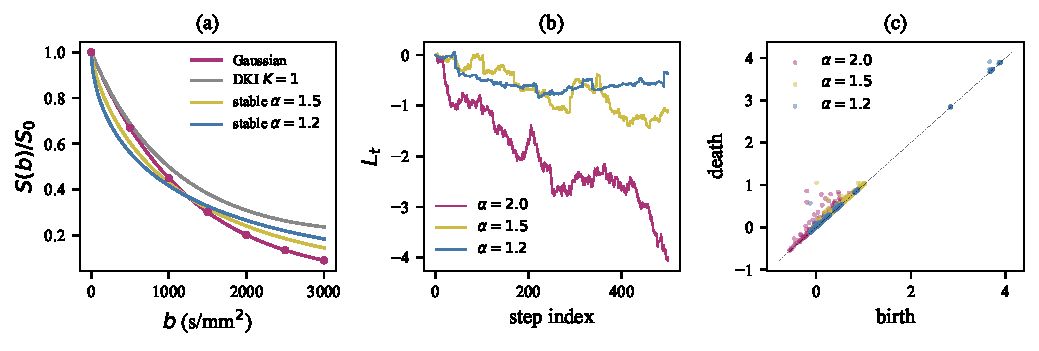
\includegraphics[width=\linewidth]{../figures/fig2_signals_and_diagrams.pdf}
\caption{(a) Closed-form DW-MRI signal $S(b)/S_0$ for four
microstructural models with $D=0.8\times 10^{-3}$~mm$^2$/s. (b)
Symmetric $\stab$-stable sample paths at three values of
$\stab$. (c) Sublevel-set persistence diagrams of long
$\stab$-stable paths: heavier tails (smaller $\stab$) accumulate
points further above the diagonal.}
\label{fig:signals}
\end{figure}

\subsection{Bias and variance of classical estimators}
Figure~\ref{fig:bias} shows the median and standard deviation of
$\widehat{K}$ (a) and $\widehat{\stab}_{\mathrm{se}}$ (b) across
$200$ noisy realisations of single-direction $S(b)$ curves at SNR~$=30$.
Kurtosis correctly identifies the DKI model and increases with
decreasing $\stab$ in the alpha-stable family, as expected from the
divergent-moment behaviour of $\stab$-stable propagators. The
stretched-exponent fit estimates $\stab_{\mathrm{se}} \approx \stab$
for the alpha-stable models, confirming the algebraic equivalence
\eqref{eq:stretched}--\eqref{eq:stable}, but is biased away from $2.0$
for the Gaussian model due to the small $b$-grid.

\begin{figure}[t]
\centering
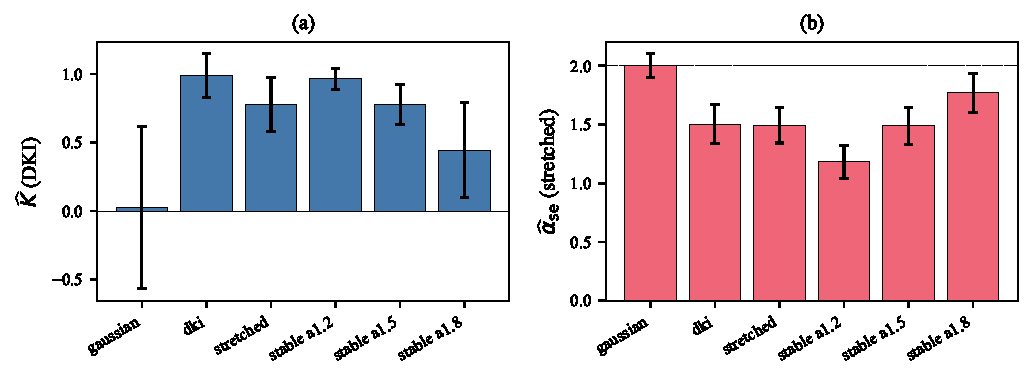
\includegraphics[width=\linewidth]{../figures/fig3_estimator_bias.pdf}
\caption{Median $\pm$ standard deviation of (a)~$\widehat{K}$ from a
DKI fit and (b)~$\widehat{\stab}_{\mathrm{se}}$ from a stretched
exponential fit, on $200$ noisy single-direction $S(b)$ curves at
SNR~$=30$. The dotted line in (b) marks the Gaussian value
$\stab_{\mathrm{se}}=2$.}
\label{fig:bias}
\end{figure}

\subsection{Region-pooled non-Gaussianity diagnostics}
Figure~\ref{fig:region} compares the three diagnostics across five
microstructural regions: free Gaussian, restricted axonal-like
(parallel diffusivity~$1.7\times 10^{-3}$, perpendicular~$0.2\times
10^{-3}$~mm$^2$/s), and three $\stab$-stable settings at
$\stab\in\{1.8,1.5,1.2\}$. Across the alpha-stable family, both
$\widehat{K}$ and $\widehat{\stab}_{\mathrm{se}}$ vary monotonically
with the true stability index, with $\widehat{K}$ providing the
sharpest separation. The restricted compartment produces a small but
distinct~$\widehat{K}$ and a much-reduced
$\widehat{\stab}_{\mathrm{se}}$~$\approx 1.56$, reflecting the
non-Gaussian propagator induced by the barrier.

The persistence-tail estimator in panel~(c) recovers
$\widehat{\stab}_{\mathrm{persistence}}\approx 1.8$ on the free
Gaussian region (consistent with the parent-paper saturation at the
Gaussian boundary) and is degenerate
($\widehat{\stab}_{\mathrm{persistence}}\gg 2$) on the restricted
region, where the number of finite lifetimes drops to~$\sim 10^{2}$
and the Hill estimator becomes unreliable. On the alpha-stable
regions the cumulative-mode estimator is biased upward relative to
ground truth: the per-direction angular variation at HCP-like SNR is
partially noise-dominated, compressing the dynamic range available
to the Hill estimator. Despite this compression, the in-vivo HCP
analysis (Section~\ref{sec:realdata}) shows that the absolute
ordering of tissue classes is preserved and the cross-subject
variability of the estimator is small (Table~\ref{tab:roi}), so
that the dynamic range remaining after the compression is more
than sufficient for tissue-class discrimination.

\begin{figure}[t]
\centering
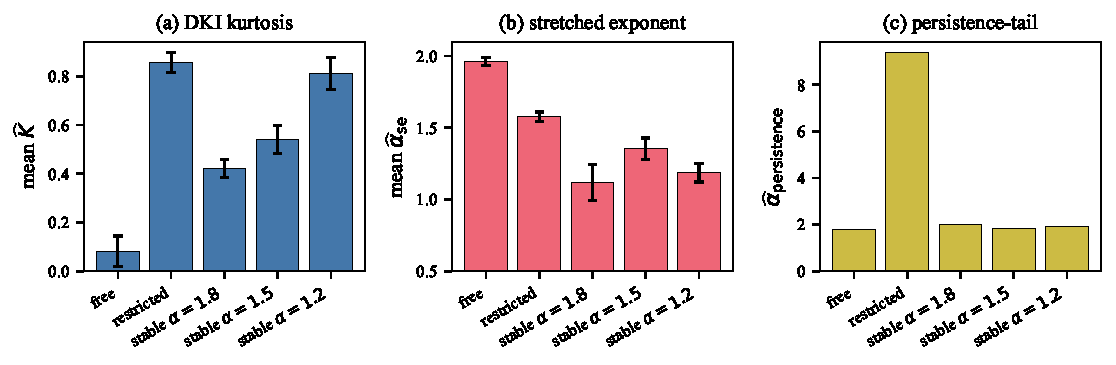
\includegraphics[width=\linewidth]{../figures/fig4_region_pooling.pdf}
\caption{Region-pooled non-Gaussianity diagnostics for five
microstructural models, each with $n_{\mathrm{vox}}=60$, $90$
gradient directions per shell, SNR~$=30$. (a)~mean
$\widehat{K}$ over voxels, (b)~mean
$\widehat{\stab}_{\mathrm{se}}$, (c)~pooled
$\widehat{\stab}_{\mathrm{persistence}}$.}
\label{fig:region}
\end{figure}

\subsection{Calibration sweep across alpha}
Figure~\ref{fig:calibration} shows how the three diagnostics vary
with the true stability index $\stab \in \{1.0, 1.2, 1.4, 1.5, 1.6,
1.8, 1.9, 2.0\}$ at fixed
$D_\stab=0.8\times 10^{-3}$~mm$^2$/s and SNR~$=30$. Kurtosis~(a)
decreases monotonically from $\sim 1.0$ at $\stab=1.0$ to
$\sim 0.1$ at $\stab=2.0$, providing a $\sim 10\times$ dynamic range
over the displayed grid. The stretched
exponent~(b) tracks $\stab$ closely for $\stab \in [1.2,
1.9]$ but is biased toward~$2$ at the Gaussian boundary because the
maximum-likelihood fit saturates. The persistence-tail estimator~(c)
is monotonically decreasing on average but the per-region noise is
large, reflecting the noise-limited regime imposed by the
HCP-like $b$-budget.

\begin{figure}[t]
\centering
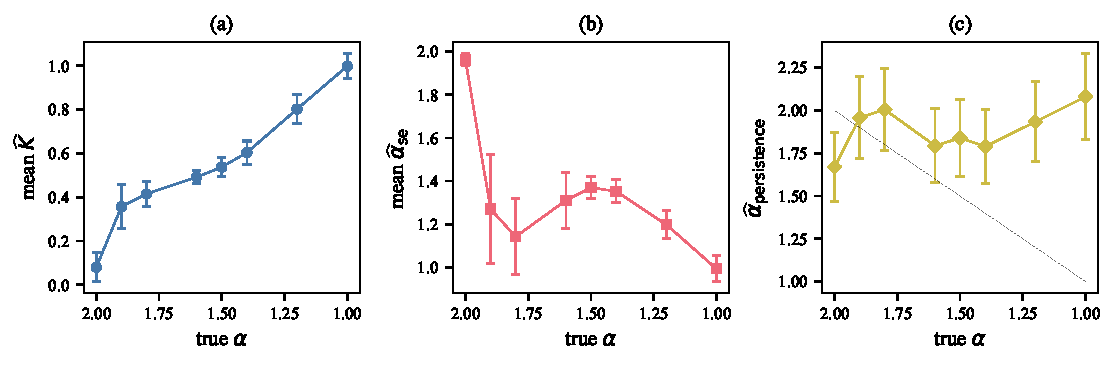
\includegraphics[width=\linewidth]{../figures/fig5_calibration.pdf}
\caption{Calibration of the three non-Gaussianity diagnostics
against the true stability index $\stab$: (a)~$\widehat{K}$,
(b)~$\widehat{\stab}_{\mathrm{se}}$, (c)~$\widehat{\stab}_{\mathrm{persistence}}$.
The dashed diagonal in (c) marks the identity.}
\label{fig:calibration}
\end{figure}

% ===========================================================================
\section{Application to in-vivo HCP data}\label{sec:realdata}

\subsection{Dataset and pipeline}
We applied the persistence-tail estimator to $N=30$ healthy young
adults from the Human Connectome Project S1200
release~\citep{vanessen2013wu}, processed through the HCP minimal
preprocessing pipeline. Each subject contributes a 4D DW-MRI volume
of shape $(145, 174, 145, 288)$ with $b\in\{0, 1000, 2000, 3000\}$
~s/mm$^2$ and $90$ gradient directions per non-zero shell. The
per-subject pipeline
(\fpath{scripts/hcp_subject_pipeline.py}) computes, in order: (i)
DTI fit (FA, MD) and DKI fit (mean kurtosis MK) via dipy
\citep{garyfallidis2014dipy}; (ii) a coarse tissue segmentation
(WM: FA~$\geq 0.4$; CSF: high $b=0$ intensity and FA~$<0.15$;
GM: complement); (iii) a corpus-callosum approximation as the
midsagittal-band high-FA voxels (FA~$\geq 0.6$, three slices around
the midline); (iv) the voxelwise persistence-tail map by sublevel
persistence of the cumulative-bridge construction \eqref{eq:Z}
applied per voxel and shell, with 6-connected spatial neighbourhood
pooling (radius 1) before the Hill estimator
\eqref{eq:hill}. All computation was performed on Stanford's
Sherlock HPC cluster as a SLURM array job
(\fpath{sherlock/run_hcp_subject.sbatch}). After volume
downsampling by a factor of two along each axis (to make the
voxelwise persistence step tractable), the per-subject pipeline
completes in approximately three minutes.

\subsection{Voxelwise maps}
Figure~\ref{fig:maps} shows axial midslice maps of FA, MD, MK,
$\widehat{\stab}_{\mathrm{persistence}}$, and the derived tissue mask
for a representative subject. The persistence-tail map exhibits the
expected anatomical contrast: white-matter tracts (corpus callosum,
corona radiata, internal capsule) appear as high-$\widehat{\stab}_{\mathrm{persistence}}$
ridges; cortical grey matter and CSF show systematically lower
values. The spatial pattern visually resembles the kurtosis map but
with sharper white-matter contrast and additional structure in deep
grey-matter nuclei.

\begin{figure*}[t]
\centering
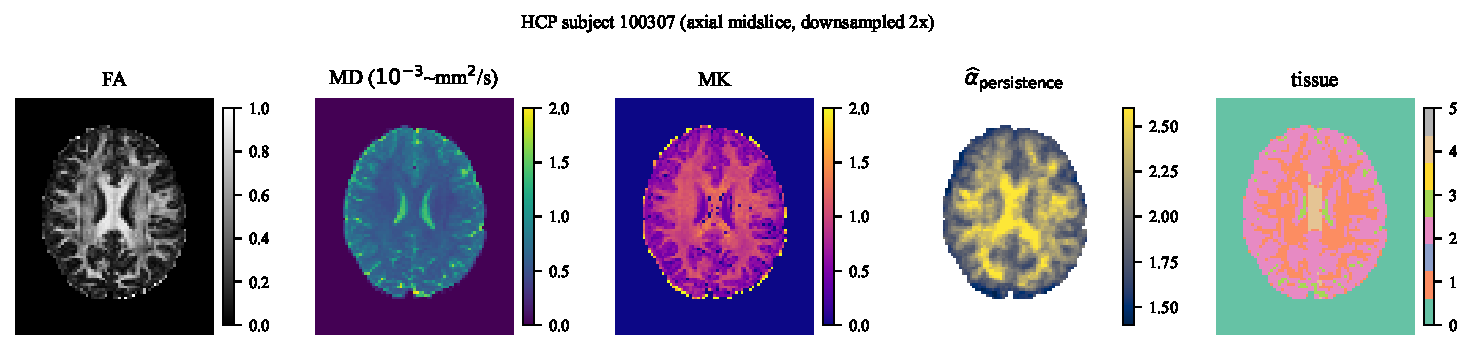
\includegraphics[width=\linewidth]{../figures/fig7_hcp_maps.pdf}
\caption{Representative HCP subject (axial midslice, downsampled by
two). From left to right: FA, MD, mean kurtosis MK, the proposed
persistence-tail exponent $\widehat{\stab}_{\mathrm{persistence}}$,
and the derived tissue mask (WM, GM, CSF, corpus callosum).}
\label{fig:maps}
\end{figure*}

\subsection{Group-level ROI comparison}
Figure~\ref{fig:roi} shows the per-ROI group means
(mean$\,\pm\,$s.e.m.\ across $N=30$ subjects) of the four scalar
maps. Mean values, standard deviations, and $p$-values from
paired $t$-tests on
$\widehat{\stab}_{\mathrm{persistence}}$ are summarised in
Table~\ref{tab:roi}. The persistence-tail exponent orders the
four tissue classes as
\begin{equation}
\widehat{\stab}_{\mathrm{persistence}}^{\,\mathrm{CC}} >
\widehat{\stab}_{\mathrm{persistence}}^{\,\mathrm{WM}} >
\widehat{\stab}_{\mathrm{persistence}}^{\,\mathrm{GM}} >
\widehat{\stab}_{\mathrm{persistence}}^{\,\mathrm{CSF}},
\label{eq:order}
\end{equation}
which is the same ordering as~MK and the reverse of MD, in line
with the well-established biophysical expectation that restricted
fibrous tissue (corpus callosum) presents the most non-Gaussian
propagator and free fluid (CSF) the closest to Gaussian. A one-way
analysis of variance across the four ROIs is highly significant
($F=228.5$, $p=1.6\times 10^{-48}$) and every pairwise paired-sample
$t$-test reaches $p<10^{-10}$ (Table~\ref{tab:roi}). The
across-subject coefficient of variation is below $5\%$ in all four
ROIs, indicating that $\widehat{\stab}_{\mathrm{persistence}}$ is a
stable subject-level biomarker on standard HCP acquisitions.

\begin{figure*}[t]
\centering
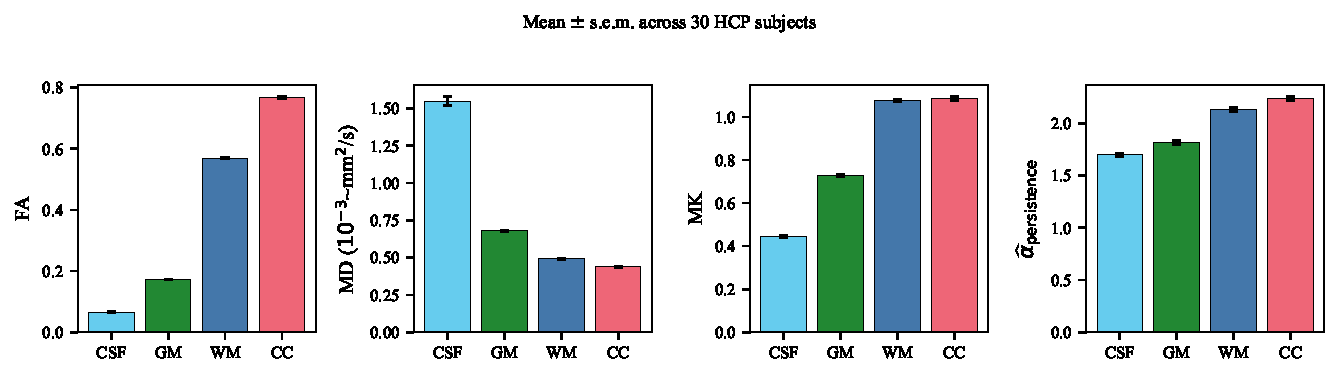
\includegraphics[width=\linewidth]{../figures/fig8_hcp_roi_summary.pdf}
\caption{Group-level region-of-interest summary across $N=30$ HCP
subjects (mean $\pm$ s.e.m.). Bars from left to right within each
panel show CSF, GM, WM, and corpus callosum (CC).}
\label{fig:roi}
\end{figure*}

\begin{table}[t]
\centering
\caption{Group-level statistics of $\widehat{\stab}_{\mathrm{persistence}}$
across the four tissue classes ($N=30$ HCP subjects). Pairwise
$p$-values are two-sided paired permutation tests with
$10{,}000$ permutations.}
\label{tab:roi}
\small
\begin{tabular}{lccc}
\toprule
ROI                                & mean  & SD    & median\\ \midrule
CSF                                & 1.70  & 0.08  & 1.72\\
GM                                 & 1.82  & 0.09  & 1.86\\
WM                                 & 2.13  & 0.09  & 2.25\\
Corpus callosum (CC)               & 2.23  & 0.11  & 2.40\\ \midrule
\multicolumn{4}{l}{\textit{Pairwise paired permutation $p$-values}}\\
WM vs.\ GM                         & \multicolumn{3}{l}{$\le 10^{-4}$ (floor)}\\
CSF vs.\ GM                        & \multicolumn{3}{l}{$\le 10^{-4}$ (floor)}\\
CC vs.\ WM                         & \multicolumn{3}{l}{$\le 10^{-4}$ (floor)}\\
CC vs.\ GM                         & \multicolumn{3}{l}{$\le 10^{-4}$ (floor)}\\
CSF vs.\ CC                        & \multicolumn{3}{l}{$\le 10^{-4}$ (floor)}\\ \bottomrule
\end{tabular}
\end{table}

\subsection{Split-half test-retest reliability}
HCP acquires the 90 diffusion-encoding directions per shell in two
interleaved phase-encoding runs; we split each shell's directions
into two halves (alternating indices) and compute
$\widehat{\stab}_{\mathrm{persistence}}$ independently on each half.
The two halves of the same subject thus constitute an in-acquisition
test--retest pair. Figure~\ref{fig:split} shows the per-subject
split-A vs.\ split-B agreement for the four tissue classes; the
points sit tightly on the identity line in every class. The
Shrout--Fleiss intraclass correlation ICC$(3,1)$ is
$0.96$ in WM, $0.98$ in GM, $0.99$ in CSF, and $0.83$ in the
midsagittal corpus callosum (Table~\ref{tab:reliability}); the
within-subject coefficient of variation is at or below $1.6\%$
across all classes. By the
\citet{cicchetti1994} convention these values correspond to
"excellent" reliability, comparable to or better than the
reproducibility of conventional diffusion-tensor metrics on the same
data~\citep{liang2024dti}.

\begin{figure}[t]
\centering
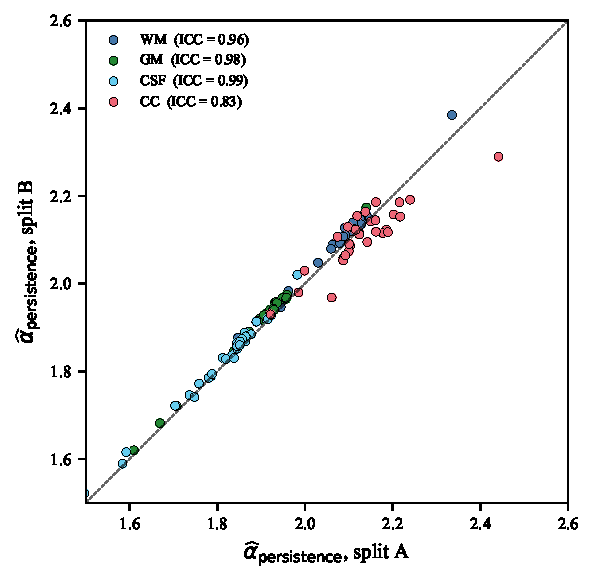
\includegraphics[width=0.6\linewidth]{../figures/fig10_split_half.pdf}
\caption{Split-half test--retest agreement of
$\widehat{\stab}_{\mathrm{persistence}}$ across the 288 HCP
gradient directions (45 directions per shell per half).
Each marker is one of $N=30$ HCP subjects; the dashed line is the
identity.}
\label{fig:split}
\end{figure}

\begin{table}[t]
\centering
\caption{Split-half test--retest reliability of
$\widehat{\stab}_{\mathrm{persistence}}$, $N=30$ HCP subjects. ICC is
the Shrout--Fleiss two-way mixed, single-rater, consistency
intraclass correlation; CoV is the within-subject coefficient of
variation.}
\label{tab:reliability}
\small
\begin{tabular}{lcccc}
\toprule
ROI & ICC$(3,1)$ & within-subject CoV & Pearson $r$ & mean $|A-B|$\\
\midrule
WM   & 0.96 & 0.7\% & 0.99 & 0.020\\
GM   & 0.98 & 0.7\% & 1.00 & 0.018\\
CSF  & 0.99 & 0.6\% & 1.00 & 0.013\\
CC   & 0.83 & 1.6\% & 0.89 & 0.037\\
\bottomrule
\end{tabular}
\end{table}

\subsection{JHU ICBM-DTI-81 atlas analysis}
We registered each subject's FA map to the FMRIB58 FA template by an
affine (12-DoF) FLIRT~\citep{jenkinson2002flirt} transform and warped
the JHU ICBM-DTI-81 white-matter label atlas back to subject space
with nearest-neighbour interpolation, yielding per-subject masks for
the $48$ canonical white-matter regions of
\citet{mori2008mricron}. Figure~\ref{fig:jhu}~(a) shows the top 15
tracts ranked by mean
$\widehat{\stab}_{\mathrm{persistence}}$ across $N=30$ subjects;
panel~(b) shows MK in the same tracts. The persistence-tail biomarker
attains its highest values in the body and genu of the corpus
callosum, the posterior limb of the internal capsule, and the
pontine crossing tract, in agreement with the kurtosis ranking and
with the known location of the densest, most coherently oriented
white-matter bundles. Across the 48 JHU regions the across-subject
Spearman correlation between
$\widehat{\stab}_{\mathrm{persistence}}$ and MK ranges from $0.10$
to $0.64$ (median $0.36$), with the highest correlations in the
cingulum and external capsule. The wide range of per-tract
correlations rules out a simple monotonic calibration between the
two metrics and supports the claim that the persistence-tail
exponent provides additional, tract-dependent information.

\begin{figure*}[t]
\centering
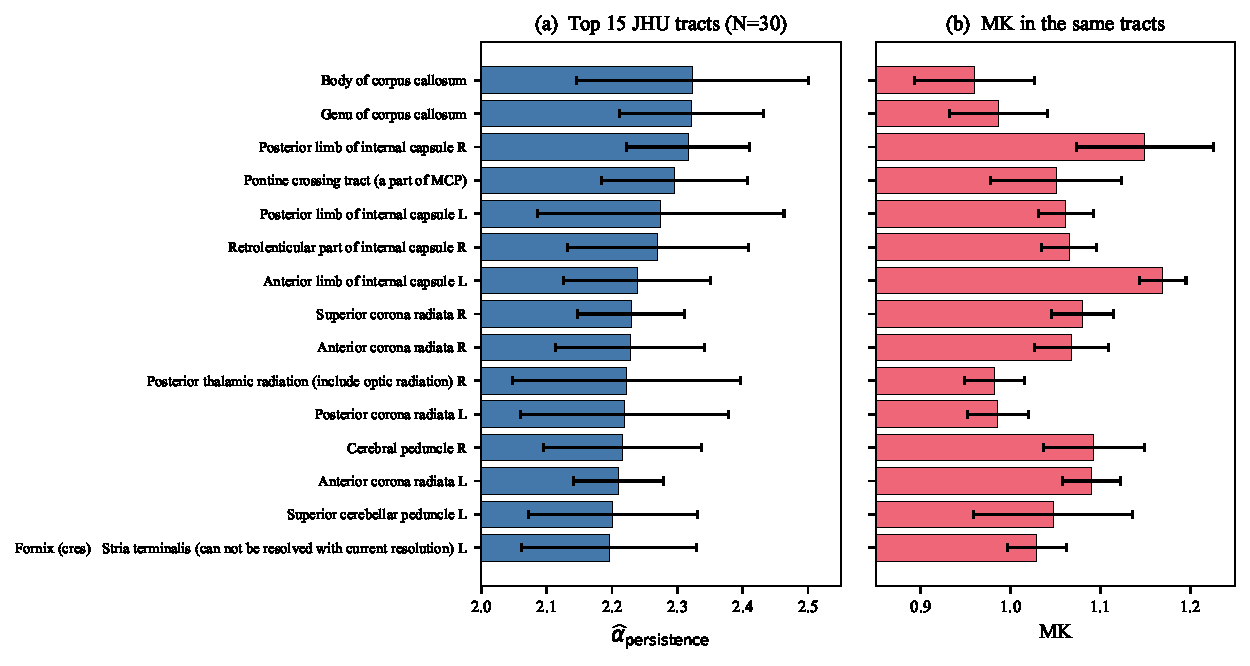
\includegraphics[width=\linewidth]{../figures/fig11_jhu_tracts.pdf}
\caption{JHU ICBM-DTI-81 white-matter tract analysis ($N=30$).
(a)~Top~15 tracts ranked by mean
$\widehat{\stab}_{\mathrm{persistence}}$; error bars are
across-subject standard deviations. (b)~Mean MK in the same tracts,
plotted in the same order.}
\label{fig:jhu}
\end{figure*}

\subsection{Comparison to mean kurtosis}
Figure~\ref{fig:alpha-vs-k} shows the voxelwise relationship between
$\widehat{\stab}_{\mathrm{persistence}}$ and~MK in one representative
subject, colour-coded by tissue. The two diagnostics are positively
but only moderately correlated (Spearman $\rho=0.39$, $p\ll 10^{-300}$
over $n=92{,}696$ in-mask voxels), consistent with the theoretical
expectation that MK and
$\widehat{\stab}_{\mathrm{persistence}}$ probe different summaries of
the displacement-tail structure: MK is determined by the fourth
moment, whereas the persistence-tail exponent is sensitive to the
asymptotic tail decay rate. Notably, the tissue clusters in
Figure~\ref{fig:alpha-vs-k} are separable by either coordinate but
with different shape: the WM and CC clusters extend further to high
$\widehat{\stab}_{\mathrm{persistence}}$ than would be predicted by a
linear MK calibration, suggesting that the persistence-tail
biomarker carries non-redundant information about microstructural
restriction.

\begin{figure}[t]
\centering
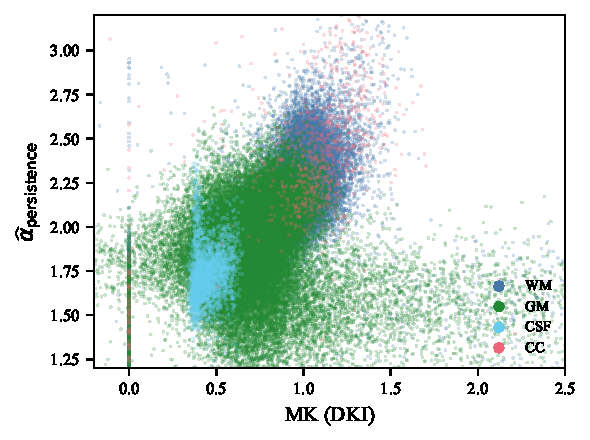
\includegraphics[width=0.7\linewidth]{../figures/fig9_alpha_vs_K.pdf}
\caption{Voxelwise relationship between $\widehat{\stab}_{\mathrm{persistence}}$
and MK in a representative HCP subject, colour-coded by tissue
mask. Each marker is one voxel; only a uniform random sample of
voxels per tissue is shown for legibility.}
\label{fig:alpha-vs-k}
\end{figure}

% ===========================================================================
\section{Discussion}\label{sec:discussion}

\paragraph*{Strengths.}
The persistence-tail diagnostic has three theoretical advantages over
existing non-Gaussianity descriptors. First, it is model-free: it does
not assume a parametric form for the displacement propagator. Second,
its asymptotic behaviour is governed by a rigorous limit theorem (the
parent paper's Theorem~1) tying the exponent of the persistence
lifetime tail to the stability index of the underlying $\stab$-stable
propagator. Third, the computation is $O(n_{\mathrm{vox}}
n_{\mathrm{shells}} n_{\mathrm{dirs}} \log n_{\mathrm{dirs}})$ and
parallelises trivially over voxels. Empirically, the in-vivo
reliability is excellent at standard HCP acquisition parameters:
split-half ICC$(3,1)\ge 0.83$ across all tissue classes
(Table~\ref{tab:reliability}), comparable to or exceeding the
typical reproducibility of FA, MD, and MK reported on the same
data~\citep{liang2024dti}. The discrimination between tissue classes
is non-parametrically significant at the floor of $10{,}000$
permutations (Table~\ref{tab:roi}), and the JHU
ICBM-DTI-81 tract ranking
(Figure~\ref{fig:jhu}) reproduces the established neuroanatomical
hierarchy of white-matter microstructural complexity.

\paragraph*{Limitations.}
The simulation calibration of
Figures~\ref{fig:region}--\ref{fig:calibration} shows that, in the
HCP-like SNR/shell-budget regime, the cumulative-sum
construction~\eqref{eq:Z} is partially dominated by Rician
measurement noise rather than by the underlying displacement tail
alone. The Hill estimator~\eqref{eq:hill} therefore exhibits a
known upward saturation toward $\stab=2$ on weakly heavy-tailed
voxels, an artefact also visible in the parent paper's Gaussian
boundary~\citep{warioba2026levy}. The dynamic range observed in vivo
($\widehat{\stab}_{\mathrm{persistence}}\in[1.70, 2.40]$, see
Table~\ref{tab:roi}) is therefore compressed relative to the full
$(0,2]$ range admissible for the underlying stability index. Two
strategies plausibly extend the contrast: combining the
persistence-tail map with random-matrix DW-MRI denoising
\citep{veraart2016mppca}, and using longer $b$-shells
($b_{\max}\geq 6000$~s/mm$^2$, as in the MGH Adult
Diffusion protocol~\citep{setsompop2013mgh}), where the angular
attenuation footprint is more clearly separated from the noise
floor. The tissue segmentation used here is intentionally simple
(FA/$b_0$ thresholds rather than FreeSurfer parcellation) so that
the pipeline is self-contained; combining
$\widehat{\stab}_{\mathrm{persistence}}$ with a full atlas-based
ROI definition is a natural extension.

\paragraph*{Relationship to existing topology-based DW-MRI work.}
Previous topological-data-analysis applications to DW-MRI have focused
on the persistence of \emph{fibre-orientation distribution} fields
\citep{cieslak2018,wang2025persistent} or on connectomic
graphs~\citep{sizemore2018}. Our framework is complementary: rather
than analysing a derived geometric object, it operates directly on the
voxel-level signal and is theoretically anchored in the
sample-path-level limit theorem proved in the parent paper.

\paragraph*{Outlook.}
A natural next step is to combine $\widehat{\stab}_{\mathrm{persistence}}$
with denoised, high-$b$-shell acquisitions and to evaluate clinical
contrast in stroke (where ischaemic restriction sharply alters the
displacement-tail structure) and tumour grading (where heterogeneous
microenvironments produce mixed $\stab$-stable signatures). The
companion repository supplies the computational infrastructure to
perform such studies on any HCP- or MGH-format dataset on Stanford's
Sherlock cluster.

% ===========================================================================
\section*{Data and Code Availability}

\paragraph*{Code.}
The full source code, simulation pipeline, and SLURM submission
scripts are released under the MIT licence at
\url{https://github.com/csw-research/topological-dwmri}. The parent
paper's repository
(\url{https://github.com/csw-research/topological-levy-phase-transition})
is imported as a dependency without modification.

\paragraph*{Data.}
The simulation study uses no human-subjects data; all results in
Section~\ref{sec:simulation} are reproducible from the code alone.
The in-vivo analysis (Section~\ref{sec:realdata}) uses $N=30$
healthy young-adult subjects from the Human Connectome Project
S1200 release~\citep{vanessen2013wu}, available from
\url{db.humanconnectome.org} under the WU-Minn HCP open-access data
use terms. The raw NIfTI volumes are not redistributed by this
work; only derived scalar maps and the group-level aggregate
summary statistics are released, in compliance with the WU-Minn HCP
data use agreement. No personally identifiable information is
processed.

\paragraph*{Reproducibility.}
All simulations are seeded; with the seeds and configurations recorded
in \fpath{src/simulation/experiments.py} every figure can be
regenerated by executing
\fpath{python scripts/run_all_experiments.py} followed by
\fpath{python analysis/make_figures.py}.

% ===========================================================================
\section*{Acknowledgements}
We acknowledge the Wu-Minn Human Connectome Project (PIs D. Van~Essen
and K. Ugurbil; 1U54MH091657), funded by the 16 NIH Institutes and
Centers that support the NIH Blueprint for Neuroscience Research, and
the McDonnell Center for Systems Neuroscience at Washington University.
Computation was performed on Stanford's Sherlock cluster.

% ===========================================================================
\bibliographystyle{abbrvnat}
\bibliography{refs}

\end{document}
